% res_dataflow.tex  -- written by Harsha
\subsection{Output- vs.\ Weight-Stationary}
For a single $4\times4$ product, OS is faster (12 vs.\ 15 cycles) because
WS must first load its weights. When many rows of $A$ share the same $B$,
as when a neural-network layer is applied to a batch, WS streams them
continuously. It then needs $3N-1+M$ cycles for $M$ rows, against
$\lceil M/N\rceil\cdot 3N$ for OS (Fig.~\ref{fig:osws}a). For $M=16$ WS measures 27 cycles, against about 48 for OS (4 products at
the measured 12.06 cycles each). WS utilisation approaches 100\,\% as $M$ grows,
while OS stays at 33\,\% (Fig.~\ref{fig:osws}b). WS is also cheaper here
(859 FFs, 32 LUTs). Its PE equation $p_{out}=p_{in}+a\cdot w$ maps directly
onto the DSP48 cascade path, and it needs neither operand buffers nor a
result buffer. The costs are 32-bit vertical links instead of 8-bit ones,
the restriction that weights cannot change while rows are in flight, and
the need for an external buffer to supply $A$ rows at full rate. This
explains the TPU's choice of WS for large batched inference. OS remains
attractive when each product has new operands and results must stay local.

\begin{figure}[t]
\centering
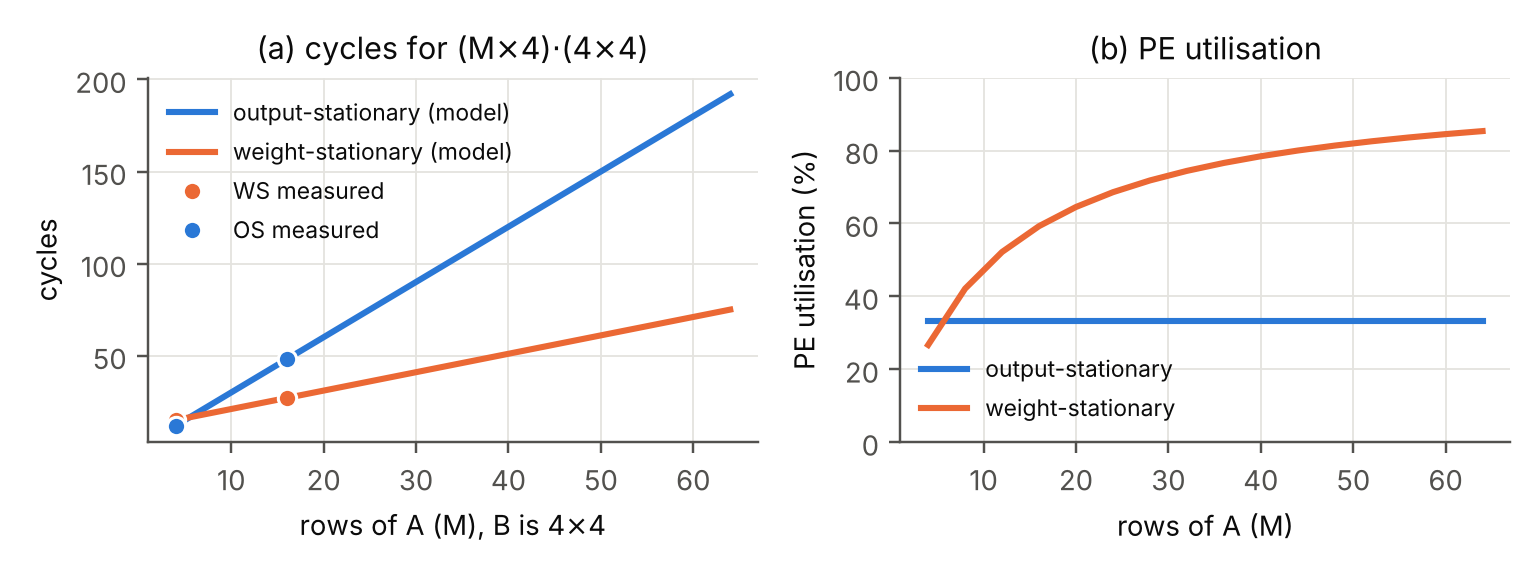
\includegraphics[width=\columnwidth]{fig_os_vs_ws.png}
\caption{OS vs.\ WS for $(M\times4)\cdot(4\times4)$: (a) cycles, (b) PE utilisation.}
\label{fig:osws}
\end{figure}
